%%%
\documentclass[mathserif, aspectratio=43]{beamer}

\usetheme{metropolis}

\metroset{progressbar=frametitle}

\usefonttheme{professionalfonts}
\usepackage{mathtools}
\usepackage{mathspec}

\makeatletter % undo the wrong changes made by mathspec
\let\RequirePackage\original@RequirePackage
\let\usepackage\RequirePackage
\makeatother

\setmathfont{Latin Modern Math}
\usepackage[none]{hyphenat}

%%% Packages section %%%
\usepackage{hyperref}
\usepackage{amsmath}
\usepackage{amsfonts}
\usepackage{tikz}
\usepackage{minted}

%%% Preamble %%%
\title{No Free Lunch}
\subtitle{Machine Learning and Data Mining}
\author{Maxim Borisyak}

\institute{National Research University Higher School of Economics (HSE)}
\usepackage{amsmath}


\begin{document}

\begin{frame}[plain]
	\titlepage
\end{frame}

\section{No free lunch}



\begin{frame}[fragile]
\frametitle{IQ test: try to learn yourself!}
First question from \href{https://www.mensa.org/workout/questions}{MENSA} website:\\
\textit{Following the pattern shown in the number sequence below, what is the missing number?}
$$1, 8, 27, ?, 125, 216$$

Possible answers:
\begin{itemize}
\item 36
\item 45
\item 46
\item 64
\item 99
\end{itemize}

\end{frame}


\begin{frame}[fragile]
\frametitle{IQ test: try to learn yourself!}
First question from \href{https://www.mensa.org/workout/questions}{MENSA} website:\\
\textit{Following the pattern shown in the number sequence below, what is the missing number?}
\begin{center}
\begin{tabular}{c | c c c c c}
$X_{\mathrm{train}}$ & 1 & 2 & 3 & 5 & 6\\
\hline
$y_{\mathrm{train}}$ & 1 & 8 & 27 & 125 & 216
\end{tabular}
\end{center}
\vspace*{5mm}
$$X_\mathrm{test} = (4, )$$


\end{frame}


\begin{frame}[fragile]
\frametitle{IQ test: try to learn yourself!}
My solution:
$$y = \frac{1}{12}(91 x^5 - 1519 x^4 + 9449 x^3 - 26705 x^2 + 33588 x - 14940)$$

\begin{itemize}
\item fits perfectly!
\end{itemize}
My answer:
\begin{itemize}
\item 99
\end{itemize}

\end{frame}


\begin{frame}[fragile]
\frametitle{IQ test}
Why solution:
$$y = x^3$$seems much more suitable than
$$y = \frac{1}{12}(91 x^5 - 1519 x^4 + 9449 x^3 - 26705 x^2 + 33588 x - 14940)?$$


\end{frame}


\begin{frame}[fragile]
\frametitle{Terminology}
Machine Learning is about learning algorithms $A$ that:
\begin{itemize}
\item defined on sample set $\mathcal{X}$ (e.g. $\mathbb{R}^n$) and targets $\mathcal{Y}$ (e.g. $\{0, 1\}$):\begin{itemize}
\item $\mathcal{X}$ and $\mathcal{Y}$ are discrete;
\end{itemize}

\item take a problem (dataset) $D = (X, y) \subseteq \mathcal{X} \times \mathcal{Y}$;
\item learn relation between $\mathcal{X}$ and $\mathcal{Y}$;
\item and return prediction function $h$ (hypothesis):
\end{itemize}
\begin{eqnarray*}
  A(D) &=& h\\
  h: \mathcal{X} &\to& \mathcal{Y}
\end{eqnarray*}
By this definition, e.g. XGBoost is a \textbf{family} of algorithms.

\end{frame}


\begin{frame}[fragile]
\frametitle{Off-training-set error}
$$\mathrm{Err}(f, h, d) = \frac{\sum_{x \in d_X} \pi(x) \mathbb{I}[ f(x) \neq h(x) ]}{\sum_{x \in d_X} \pi(x)}$$

where:
\begin{itemize}
\item $h = A(d)$;
\item $f$ - true dependency;
\end{itemize}
\vfill
\begin{quote}
In most practical cases, $\mathrm{Err} \approx \mathrm{accuracy}$.

\end{quote}

\end{frame}


\begin{frame}[fragile]
\frametitle{No free lunch, strictly}
For any two learning algorithms $A_1$ and $A_2$:
\begin{enumerate}
\item uniformly averaged over all $f$, for any $n$:
$$\mathbb{E}(\mathrm{Err} \mid f, |D| = n, A_1) - \mathbb{E}(\mathrm{Err} \mid f, |D| = n, A_1) = 0$$
\item uniformly averaged over all $f$, for any $d$:
$$\mathbb{E}(\mathrm{Err} \mid f, d, A_1) - \mathbb{E}(\mathrm{Err} \mid f, d, A_1) = 0$$
\item uniformly averaged over all priors $P(f)$:
$$\mathbb{E}(\mathrm{Err} \mid |D| = n, A_1) - \mathbb{E}(\mathrm{Err} \mid |D| = n, A_1) = 0$$
\item uniformly averaged over all priors $P(f)$, for any $d$:
$$\mathbb{E}(\mathrm{Err} \mid d, A_1) - \mathbb{E}(\mathrm{Err} \mid d, A_1) = 0$$
\end{enumerate}

\end{frame}


\begin{frame}[fragile]
\frametitle{No free lunch theorem}
No free lunch theorem states that \textbf{on average by all datasets}
all learning algorithms are equally bad at learning.\\
Examples:
\begin{itemize}
\item crazy algorithm:
$$f(x) = \left\lfloor \left( \left\lceil \sum_i x_i + \theta \right\rceil \mod 17 + 1027 \right)^\pi \right\rfloor \mod 2$$
\item any configuration of SVM
\end{itemize}
perform equally well \textbf{on average}.

\end{frame}


\begin{frame}[fragile]
\frametitle{No free lunch theorem}
\begin{figure}
\centering
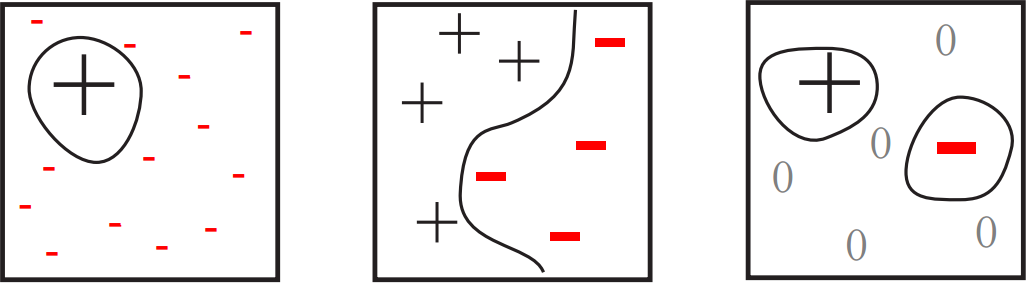
\includegraphics[width=0.8\textwidth]{imgs/no-free-lunch.png}
\end{figure}
Possible learning algorithm behaviours in \textbf{problem space}:
\begin{itemize}
\item \textbf{+} - better than the average;
\item {\color{red} \textbf{\textemdash}} - worse than the average.
\end{itemize}

\end{frame}


\begin{frame}[fragile]
\frametitle{Is Machine Learning useless?}
\begin{center}
\phantom{\Huge No.}
\end{center}

\end{frame}


\begin{frame}[fragile]
\frametitle{Is Machine Learning useless?}
\begin{center}
\textbf{\Huge No.}
\end{center}

\end{frame}


\section{Assumptions and algorithms}



\begin{frame}[fragile]
\frametitle{Is Machine Learning useless?}
No Free Lunch theorem applies to:
\begin{itemize}
\item one learning algorithm;
\item against all possible problems.
\end{itemize}
\vspace*{5mm}
In real world we have:
\begin{itemize}
\item \textbf{data scientist} with prior knowledge of the world;
\item problem description;
\item data description;
\item a set of standard algorithms.
\end{itemize}

\end{frame}


\begin{frame}[fragile]
\frametitle{Is Machine Learning useless?}
Real world problems often behave nicely:
\begin{itemize}
\item data is collected by humans (features are determined by humans);\begin{itemize}
\item algorithms with human-bias dominate (e.g. XGboost);
\end{itemize}

\item problems are posed by humans;
\item a lot of assumptions behind the data can be quickly identified from the problem domain.
\end{itemize}

\end{frame}


\begin{frame}[fragile]
\frametitle{Traditional ML (simplified)}
\begin{itemize}
\item analyze the problem and make assumptions;
\item pick an algorithm from a toolkit (e.g. logistic regression);
\item provide assumptions suitable for the algorithm (\textbf{feature engineering}).
\end{itemize}
\begin{figure}
\centering
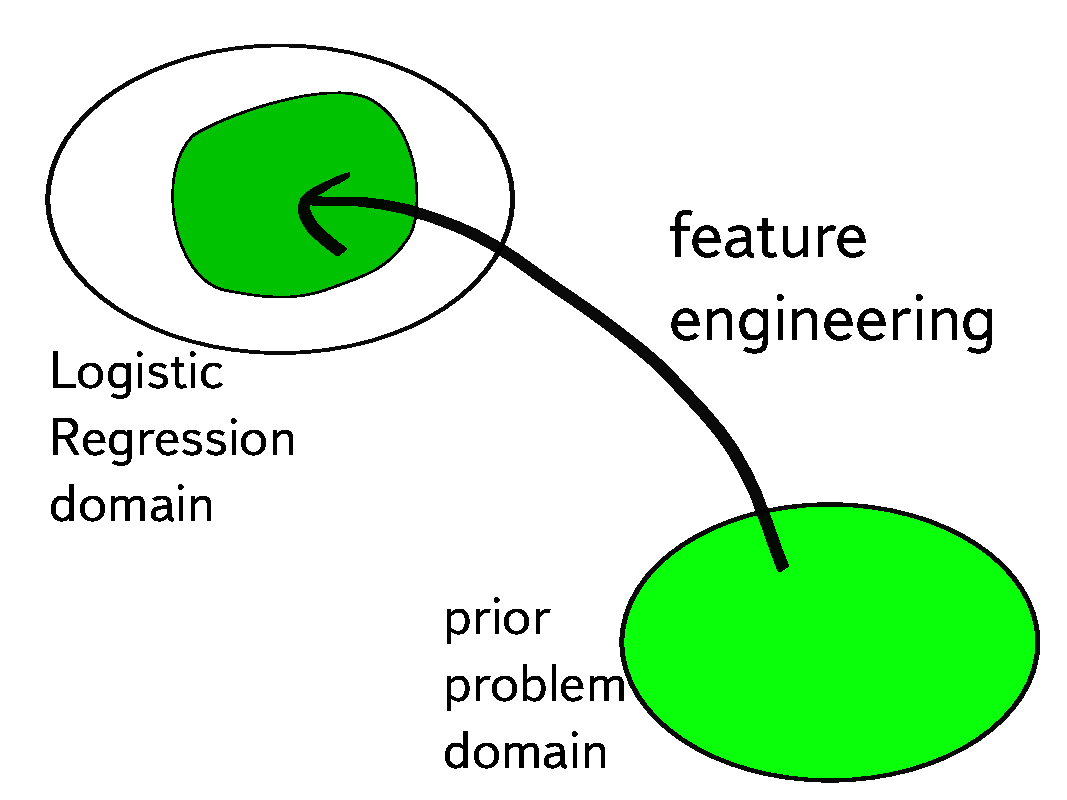
\includegraphics[width=0.42\textwidth]{/tmp/tmp1y7iamnpmdslides/mdslides/fe.pdf}

\end{figure}


\end{frame}


\begin{frame}[fragile]
\frametitle{Discussion}
\begin{itemize}
\item this approach works well for traditional datasets with a small number of features:
\item e.g. Titanic dataset:\\\begin{center}
\begin{tabular}{|c | c | c | c | c | c|}
\hline
passenger class & name & gender & age & fare & \dots\\
\hline
\end{tabular}
\end{center}

\end{itemize}
Essentially, performance of the algorithm depends on:
\begin{itemize}
\item knowledge of the domain;
\item feature engineering skills;
\item understanding of assumptions behind standard algorithms.
\end{itemize}

\end{frame}


\begin{frame}[fragile]
\frametitle{Discussion}
What are the assumptions behind:
\begin{itemize}
\item logistic regression,
\item decision trees,
\item linear SVM,
\item SVM with RBF kernel?
\end{itemize}

\end{frame}


\begin{frame}[fragile]
\frametitle{Discussion}
What about:
\begin{itemize}
\item cross-validation-based algorithm selection?
\end{itemize}

\end{frame}


\begin{frame}[fragile]
\frametitle{Discussion}
{\Large What if we consider accuracy instead of off-training-set accuracy? }
{ \Large $$\phantom{\mathrm{accuracy} = \mathrm{generalization} + \mathrm{memorization} }$$}

\end{frame}


\begin{frame}[fragile]
\frametitle{Discussion}
{\Large What if we consider accuracy instead of off-training-set accuracy? }
{ \Large $$\mathrm{accuracy} = \mathrm{generalization} + \mathrm{memorization}$$}

\end{frame}


\begin{frame}[fragile]
\frametitle{Discussion}
{\Large What about other losses? }

\end{frame}


\begin{frame}[fragile]
\frametitle{Representation matters}
\begin{columns}
\begin{column}{0.4875\textwidth}
\begin{tabular}{ c c c | c }
$x_1$ & $x_2$ & $x_3$ & $y$ \\
\hline
0 & 0 & 0 & 0\\
\hline
0 & 0 & 1 & 0\\
\hline
0 & 1 & 0 & 1\\
\hline
0 & 1 & 1 & 0\\
\hline
1 & 0 & 0 & 0\\
\hline
1 & 0 & 1 & 1\\
\hline
1 & 1 & 0 & 0\\
\hline
1 & 1 & 1 & 0\\
\end{tabular}

\end{column}
\begin{column}{0.4875\textwidth}
\begin{phantom}
a
\end{phantom}

\end{column}
\end{columns}

\end{frame}


\begin{frame}[fragile]
\frametitle{Representation matters}
\begin{columns}
\begin{column}{0.4875\textwidth}
\begin{center}
\begin{tabular}{ c c c | c }
$x_1$ & $x_2$ & $x_3$ & $y$ \\
\hline
0 & 0 & 0 & 0\\
\hline
0 & 0 & 1 & 0\\
\hline
0 & 1 & 0 & 1\\
\hline
0 & 1 & 1 & 0\\
\hline
1 & 0 & 0 & 0\\
\hline
1 & 0 & 1 & 1\\
\hline
1 & 1 & 0 & 0\\
\hline
1 & 1 & 1 & 0
\end{tabular}
\end{center}
$$x = 4\cdot x_1 + 2\cdot x_2 + x_3 $$


\end{column}
\begin{column}{0.4875\textwidth}
\begin{center}
\begin{tabular}{ c | c }
$x$ & $y$ \\
\hline
0 & 0\\
\hline
1 & 0\\
\hline
2 & 1\\
\hline
3 & 0\\
\hline
4 & 0\\
\hline
5 & 1\\
\hline
6 & 0\\
\hline
7 & 0
\end{tabular}
\end{center}
$$y = \begin{cases} 1,& x \mod 3 = 2;\\ 0, &\text{otherwise} \end{cases}$$


\end{column}
\end{columns}

\end{frame}


\begin{frame}[fragile]
\frametitle{Representation matters}
Solve with a descent algorithm:
$$(x - 8) ^2 \to \min$$where: $x \in \{0, 1, \dots, 15\}$
\begin{itemize}
\item $\mathrm{neighbors}(x) = x \pm 1$;
\item $\mathrm{neighbors}(x) = \left\{ z \mid  \|\mathrm{binary}(x) - \mathrm{binary}(z)\|_1 = 1 \right\}$
\end{itemize}

\end{frame}


\section{Algorithms}



\begin{frame}[fragile]
\frametitle{Quiz}
\begin{center}
\textbf{ \Large What makes a good family of learning algorithms (ML library)?}
\end{center}

\end{frame}


\begin{frame}[fragile]
\frametitle{Corollary from No-Free-Lunch}
\vspace*{5mm}
A good machine learning family of algorithms/framework:
\begin{itemize}
\item has clear relation between hyperparameters and set of problems each algorithm covers.
\end{itemize}
\vspace{5mm}
A great machine learning family/frameworks:
\begin{itemize}
\item covers a wide range of problems;
\item but each algorithm covers a small set of problems;
\item i.e. a lot of sensitive and well-defined hyperparameters.
\end{itemize}
\vspace{5mm}
\textit{Here feature engineering/selection/generation is a part of the algorithm.}

\end{frame}


\begin{frame}[fragile]
\frametitle{I just leave it here}
\begin{figure}
\centering
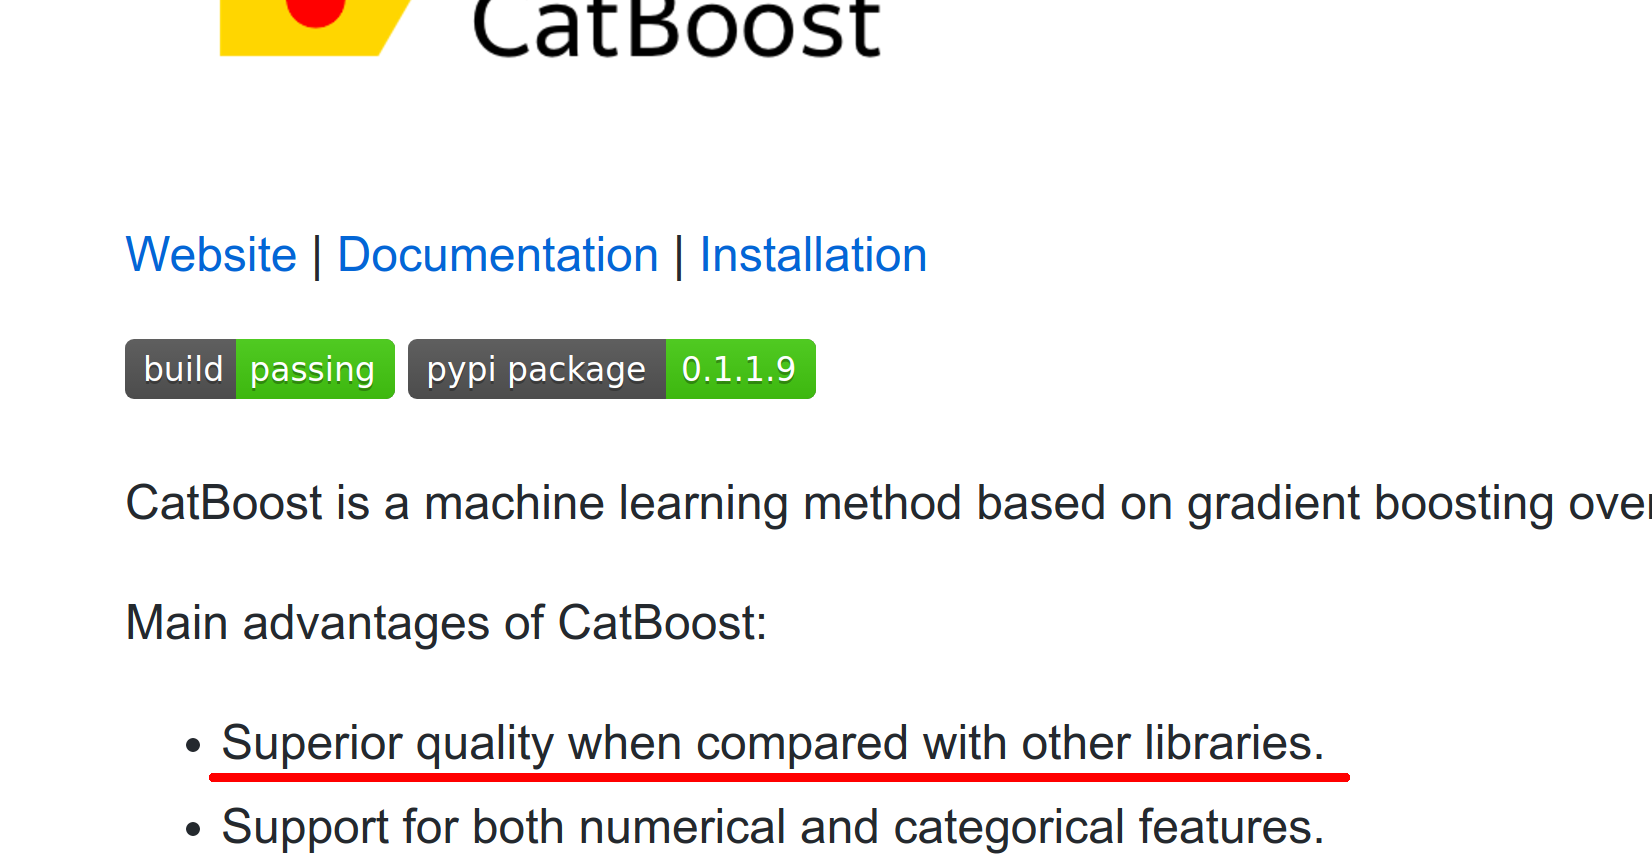
\includegraphics[width=1\textwidth]{/tmp/tmp1y7iamnpmdslides/mdslides/catboost.png}

\end{figure}


\end{frame}


\section{Summary}



\begin{frame}[fragile]
\frametitle{Summary}
No-Free-Lunch:
\begin{itemize}
\item learning is impossible without prior knowledge;
\item there is no silver bullet for learning;
\item every learning algorithm has assumptions behind it;
\item \textbf{data scientist's} job is to select/make an algorithm to match the assumptions.
\end{itemize}

\end{frame}


\begin{frame}[fragile]
\frametitle{References}
No-Free-Lunch theorem:
\begin{itemize}
\item Schaffer, Cullen. "A conservation law for generalization performance." Proceedings of the 11th international conference on machine learning. 1994.
\item Wolpert, David H. "The supervised learning no-free-lunch theorems." Soft computing and industry. Springer London, 2002. 25-42.
\item Wolpert, David H., and William G. Macready. "No free lunch theorems for optimization." IEEE transactions on evolutionary computation 1.1 (1997): 67-82.
\end{itemize}

\end{frame}

\end{document}
